\documentclass[a4paper]{article}
\usepackage[utf8]{inputenc}  % For encoding, especially for special characters
\usepackage{graphicx}
\usepackage{ulem}
\usepackage{soul} 
\usepackage{changepage} % add this in your preamble
\usepackage[a4paper, left=1in, right=1in, top=1in, bottom=1in]{geometry}
% Ensure hyperlinks are blue
\usepackage[
  colorlinks=true,   % Enable color for links
  linkcolor=blue,    % Set color of internal links
  urlcolor=blue,     % Set color of URL links
  filecolor=blue,    % Set color of file links
  citecolor=blue     % Set color of citation links
]{hyperref}

\begin{document}


\includegraphics[width=0.73668in,height=0.81548in]{media/image1.png}
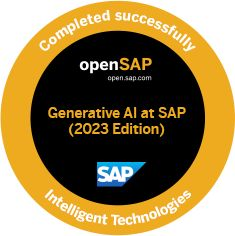
\includegraphics[width=0.74287in,height=0.74561in]{media/image2.jpeg}

\includegraphics[width=0.62821in,height=0.87111in]{media/image3.png}

\includegraphics[width=0.87421in,height=0.92262in]{media/image4.png}

\includegraphics[width=0.60088in,height=0.8017in]{media/image5.png}

\includegraphics[width=0.99074in,height=1.01661in]{media/image6.png}

\includegraphics[width=0.65064in,height=0.65064in]{media/image7.png}

\begin{center}
  {\large \textbf{Mujahed H.}}\\[0.2cm]
\end{center}
\begin{center}
  \textbf{(Gen AI/Agentic AI Data Cloud Lateral Trainer)}
\end{center}
\begin{center}
  \href{mailto:mujahed.trainer@gmail.com}{mujahed.trainer@gmail.com} \textbar{} +91 00 0000 1234
\end{center}

\rule{\textwidth}{0.4pt}


As an experienced data platform architect and training professional with
over \textbf{22 years} of experience in online, onsite, and corporate
training, I have developed a strong proficiency in analyzing and
interpreting large and complex data sets. My ability to discover
valuable patterns enables me to provide insightful answers to business
questions and identify new opportunities. I am skilled in leveraging
machine learning algorithms, cloud computing, visualization, and big
data environments to make bold, data-driven decisions. My passion for
teaching and training has allowed me to deliver high-quality training
sessions that inspire and empower learners to achieve their goals.


\begin{center}
  \textbf{SUMMARY}
  \rule{\textwidth}{0.4pt}  % Full width of the page
\end{center}


\begin{itemize}
\item
  Passionate about design data architect \& crunching System.
\item
  Excellent leadership and organizational skills
\item
  Worked with different Lang Chain language Models (N-gram, statistical,
  neural, Pretrained, fine-tuning, Evaluation of Language Models)
\item
  Strong architecture, analytical and logical reasoning
\item
  Able to work in deadline-oriented environment
\item
  Designing, implementing, and managing cloud-based big data solutions
  enables me to impart practical, hands-on knowledge to learners.
\item
  A strong believer in cutting edge technology and providing smart
  solutions.
\item
  Logically optimized solution through coding and implementation.
\item
  Diligent team player with sound analytical skills of self-defining
  performance parameters
\item
  Ability to objectively evaluate results.
\end{itemize}

\begin{center}
  \textbf{SKILLS}
  \rule{\textwidth}{0.4pt}  % Full width of the page
\end{center}

\textbf{Programming:}


\begin{quote}
\textbf{Python:}

\begin{adjustwidth}{1.2cm}{} % <-- adds left indentation
Language Specifications (Control Flows, Functions, Modules). List
comprehensions, lambda, Generators, iterators, context manager, OOP
(Multiple Inheritance and Method Resolution Order, Abstract Base Classes
(ABCs) and Interfaces, Operator Overloading and Special Methods,
Descriptors and Properties, Class Decorators and Meta classes, Mixin
Classes and Composition, Dynamic Class Creation and Modification, Slots
and Memory Optimization, Design Patterns and OOP Principles), Mockito.

\ul{Package NumPy} — Array creations, manipulation, universal functions,
operations, iteration, masking filtering, linear algebra operations,
masked arrays, memory management, performance optimization like
vectorization, indexing, slicing, broadcasting, mathematical functions.

\ul{Package Pandas} — Series, data frames, indexing, selecting data,
data cleaning, manipulation, grouping and aggregating, time series
analysis, IO operations (csv, JSON, parquet), performance optimization,
handling categorical data, reshape \& pivot tables, combining data,
time zone handling, pandas extensions, advanced data manipulation,
outliers \& anomalies, parallel processing, debugging \& best practices.

\ul{Package Matplotlib \& Seaborn} — Creating plots, charts, graphs.

\ul{Scikit-learn Package} — Data handling, supervised learning
algorithms, clustering, PCA, model evaluation and selection,
cross-validation, metrics for model evaluation, model hyperparameter
tuning using grid and random search.
\end{adjustwidth}

\vspace{0.2cm}

\textbf{Scala \& R:}

\begin{adjustwidth}{1.2cm}{} % same indentation for consistency
Classes \& Objects, Language Specifications, Closures, Collections,
Traits, Patterns, RegEx, Extractors, File IO, Packages, OOPs, Params
Types, Exceptions, Map, Annotations, Options, Evaluations, Streaming,
Serializations, etc.
\end{adjustwidth}

\vspace{0.2cm}

\textbf{Other Programming Languages:}

\begin{adjustwidth}{1.2cm}{} % indent again
JSON, Markdown, YAML, XML.
\end{adjustwidth}
\end{quote}

No Code Platform:

\textbf{N8N(Node In Node)}

\begin{quote}
\textbf{Execution \& Flow Control}: Split In Batches, Merge (Wait/Append
Mode), Wait, If, Switch, Error Workflow, Continue On Fail, Execute
Workflow, Run Once for Each Item

\textbf{Scripting \& Logic}: Function, Function Item, JavaScript, Item
Looping, Dynamic Routing, Custom Expressions, Dot Notation, Paired
Items, Chained Executions

\textbf{Data Handling}: Binary Data, Base64, Buffer, Data Mapping,
Expression Editor, Data Nesting, Flatten JSON, Regex, Templating,
JSON.parse/stringify

\textbf{Authentication \& Security}: OAuth2, JWT, API Key, Basic Auth,
HMAC, Header Validation, Credential Encryption, Environment Variables,
Vault

\textbf{Custom \& Extensibility}: Custom Nodes, Community Nodes, Node
Dev CLI, Custom Modules, Webhook Testing, External APIs, Custom
Credentials, TypeScript Node Dev

\textbf{Deployment \& Configuration}: Docker, Kubernetes, PostgreSQL,
Redis, Worker Mode, Queue Mode, Scaling, Load Balancing, n8n CLI,
Webhooks Tunneling, Multi-tenant

\textbf{Monitoring \& Debugging}: Execution Logs, Workflow Metrics, Node
Timing, Manual Debugging, Custom Error Paths, Trigger Replay, UI
Snapshots, Log Streaming

\textbf{Versioning \& Integration}: Workflow Versioning, Git Sync, JSON
Export, Import via API, n8n API, Persistent Storage, Shared Workflows,
Parameter Linking
\end{quote}

\textbf{LangFlow}:

\begin{quote}
\textbf{Core Concepts:} Chains, Agents, Tools, Components, Nodes,
Graphs, Flow Canvas, Dynamic Routing

\textbf{Models \& Backends:} LLM, OpenAI, Anthropic, Mistral, Ollama,
LangChain, Custom Endpoints

\textbf{Data Handling}: Memory, Buffers, Retrieval, Vector Stores,
Embeddings, Chroma, FAISS, Weaviate

\textbf{Custom Logic \& Programming}: Prompt Templates, Custom Tools,
Tool Calling, Function Calling, Python Code Node, Conditionals, Routing
Logic

\textbf{Agent Control}: Tool Executor, ReAct, Conversational Agent, Tool
Selection, Tool Abstraction, Memory Management, Agent Executor

\textbf{UI/UX \& Visualization}: Drag-and-Drop, Node Parameters,
Input/Output Preview, Live Debugging, Flow Execution Viewer, Session
Tracking

\textbf{Integration \& Extensibility}: API Calls, Custom Components,
Third-Party Tools, Webhook Integration, LangChain Hub, External APIs

\textbf{Deployment \& Hosting}: Docker, Self-Hosting, Streamlit, FastAPI
Backend, Local Models, GPU Support

\textbf{Security \& Configs}: API Keys, Environment Variables, CORS,
Auth Middleware, Custom Config Files

\textbf{Utilities \& Misc}: Streaming, Callbacks, Logging, Caching,
Batch Processing, Async Support, Flow Saving/Loading
\end{quote}

\textbf{Core \& Adv. Machine Learning:}

\begin{quote}
Math \& Statistics:

Linear Algebra, derivatives and gradients, distributions and hypothesis
testing.

Data Processing \& Feature Engineering:

Handling missing data and outliers, Feature selection and extractions,
Normalization, Scaling of features.

\textbf{Supervised Algorithms}: Linear Regression, Logistic Regression,
Decision Tree, Random Forests, SVM (Support Vector Machine), Naïve Bayes
Classifiers, KNN (K-Nearest Neighbors).

\textbf{Unsupervised Algorithms}: Clustering (K-Means, Hierarchical
Clustering), Dimensionality reduction Techniques (PCA- Principal
Component Analysis, t-SNE)
\end{quote}

\textbf{Reinforcement Learning}

\textbf{Natural Language Processing (NLP):}

\begin{quote}
\textbf{Topic Modeling}: Latent Dirichlet Allocation (LDA), Latent
Semantic Analysis (LSA), Non-negative Matrix Factorization (NMF),
Hierarchical Dirichlet Process (HDP)

\textbf{Word Embeddings}: Word2Vec, GloVe (Global Vectors for Word
Representation), FastText, Doc2Vec

\textbf{Sequence Labeling}: Named Entity Recognition (NER),
Part-of-Speech (POS) Tagging, Chunking \& Shallow Parsing

\textbf{Dependency Parsing}: Dependency grammar, Transition-based and
graph-based parsing algorithms, Parsing techniques like Arc-standard,
Arc-eager, and more

\textbf{Advanced Text Classification}: Hierarchical classification,
multi-label classification, Ensemble methods for text classification

\textbf{Sentiment Analysis}: Aspect-based sentiment analysis,
Fine-grained sentiment analysis, Handling negation and sarcasm

\textbf{Syntax and Grammar}: Context-Free Grammar (CFG), Probabilistic
Context-Free Grammar (PCFG), Parsing with CFGs and PCFGs

\textbf{Machine Translation}: Statistical Machine Translation (SMT),
Neural Machine Translation (NMT), Phrase-based translation models
\end{quote}

\textbf{Information Extraction}: Relation extraction, Event extraction,
Template-based extraction

\begin{quote}
\textbf{Coreference Resolution}: Anaphora and cataphora resolution,
Mention detection, Resolution algorithms

\textbf{Semantics and Ontologies}: Semantic Role Labeling (SRL), Frame
Semantics, WordNet and other lexical databases, Ontology-based NLP

\textbf{Dialogue Systems}: Intent recognition, Slot filling, Dialog
state tracking, Reinforcement learning for dialogue management
\end{quote}

\textbf{Generative Artificial Intelligence (GenAI):}

\begin{quote}
Generative AI, Variational Auto Encoders (VAE), GAN, Auto-regressive
model, flow-based model, energy-based model, Text Generation, NLP with
GPT-3, MLOps, MLFlow, LLM (H2O Studio, LangChain, GPT4), Probabilistic
Modeling, Parametric \& Non-parametric Models, Generation and Sampling
techniques, Dagshub, Vector Database, Flask Gen AI Model Deployment,
DVC.
\end{quote}

\textbf{GenAI Platform (H2O.ai):}

\begin{quote}
In-Memory machine, AutoML, MLOps, GenAI Models (Building, Predicting,
Adding Layers), Gradient Boosting Machine Model, Hyperparameter tuning
using grid search, XGBoost and Deep Learning Models, handling Time
series analysis, NLP with Sentiment analysis experiment setup
configuration, etc.
\end{quote}

\textbf{GenAI Platform (Meta LLAMA3, Hugging face):}

\begin{quote}
Architecture text generation methods, optimizing generative models for
different applications, Generative Adversarial Network (GAN) in image
and video synthesis, Integrating LLMs with other AI Models for
multimodal tasks, etc.
\end{quote}

\textbf{Prompt Engineering:}

\begin{quote}
GenAI, LLM, NLP, NER (Named Entity Recognition), Model techniques \&
Fine tunings, Prompting Strategies, Few \& Zero shot learning,
Hyperparameter tuning, Future trends \& research directions.
\end{quote}

\textbf{GenAI- Generative Artificial Intelligence with Integrations
(Application Integrations):}

\begin{itemize}
\item
  Microsoft Excel Integrations

  \begin{itemize}
  \item
    Data Analysis and Insights
  \item
    Automating Repetitive Tasks
  \end{itemize}
\item
  AI in Presentation Tools (Google Slides/Microsoft PowerPoint)

  \begin{itemize}
  \item
    Design Assistance
  \item
    Content Generation
  \end{itemize}
\item
  AI in Email Management

  \begin{itemize}
  \item
    Prioritizing and Drafting Responses
  \end{itemize}
\item
  AI in Scheduling and Calendar Management
\item
  AI in Market and Customer Insights
\item
  Analyzing Customer Feedback
\item
  Predictive Analytics
\item
  AI in Content Creation and Marketing
\item
  Strategic Implementation of Generative AI
\item
  Identifying Opportunities for AI Integration
\end{itemize}

\textbf{SQL \& PL/SQL:}

\begin{quote}
SQL, DML, DDL, SQL Operators, Joins, Sub Queries, Trigger, Cursor,
Exceptions, Functions, procedures, Indexes, Sequences, Views \& Others
Database Objects.
\end{quote}

\textbf{Multi Cloud Technologies}:

\textbf{AWS}

\begin{quote}
\textbf{Compute}: EC2, Elastic Load Balancer, Elastic Beanstalk, Lambda,
ECS and EKS.

\textbf{Storage}: EBS, S3, Glacier, EFS, Instance Store, Storage
Gateway.

\textbf{Management:} CloudFormation, CloudWatch, Cloud Trial, AWS Auto
Scaling.

\textbf{Networking:} VPC, API Gateway, IAM, Security Group, Route53.

\textbf{Data platform:} RDS, NoSQL-DynamoDB, Glue (ETL), AWS Snowflake,
Redshift.

\textbf{Machine Learning:} Translate, SageMaker, Comprehend, Lex, Polly,
Rekognition, MLOps and MLFlow.

\textbf{Analytics:} Athena, Big Data, EMR (Hadoop, Spark), Kinesis,
Quick Sight (BI).

\textbf{Development:} Code Commit, Code Pipeline, Code Whisperer,
Cloud9.

\textbf{Others:} AWS Amplify, SNS, SQS and Step Functions.
\end{quote}

\textbf{Azure:}

\begin{quote}
\textbf{Compute}: Virtual Machine.

\textbf{Storage}: Blob Storage.

\textbf{AI/ML:} MLOps, Azure Machine Learning, MLFlow, Azure Databricks
for Data Science, Data Lake, Delta Lake, Lake house, Azure ML Pipeline,
Azure ML Deployment on AKS.

\textbf{Big Data:} HDInsight, Data Bricks.

\textbf{Migration}: On-Prem to Azure migration, Data Migration Service,
Server \& Database Migration, SQL Server Azure to Azure Multi Account
migration.

\textbf{Big Data:} HDInsight, Data Bricks.

\textbf{Azure DevOps (VSTS):} Azure Boards (Kanban boards), Azure
Pipeline (Kubernetes, YAML), Azure Repo (Repo \& Github), Azure Test
Plans, Azure Artifacts and also deployed Complete End to end Application
in Python.

\textbf{Other Services}: Microsoft IIS, Virtual Net (VNet), IAM
(Identity and Service Providers), PaaS Services, Azure Active Directory,
SSO, OAuth, MFA-Multi Factor Authentication, Directory Service, Domains.

\textbf{Certification}: Microsoft Azure AZ-104, Azure Developer
Associate, AI-900, AZ-400 Azure DevOps Engineer, DP-100, DP203.

\textbf{GCP-Google Cloud Platform}:

\textbf{Compute}: Compute Engine Advance Features (Confidential VM,
Managed AD, Migrate), Migrate to VM, App Engine GKE and Cloud Functions.

\textbf{Storage \& BigData}: Cloud Storage, Cloud SQL, Dataflow, IoT
Core, Databricks, Big Query, Spark.

\textbf{Cloud AI}: Speech API, DailogFlow/api.ai (NLU, Chat \& Voice
Bots).

\textbf{Apigee Services}: Apigee X, Apigee Hybrid, Apigee Edge, Apigee
Edge Private Cloud/OPDK, Apigee Micro gateway, Apigee Adapter for Envoy.

\textbf{Anthos Services}: GKE, Anthos Deployment Models (AWS, Azure,
Bare Metal, VMware), Anthos Config Management, Cloud Marketplace and
Deploy Cloud Run for Anthos, Cloud Volumes by NetApp

\textbf{Networking}: VPC, KMS, Load Balancing, CDN, DNS, Firewall Rules,
VPN.

\textbf{Cloud AIML \& APIs}: Vertex AI, Vision, Translate, Natural
Language, CloudML, Speech API, DialogFlow/api.ai (NLU, Chat \& Voice
Bots).

\textbf{Management}: Cloud Console, Logging, Debugger \& Monitoring.

\textbf{Security Services}: GCP Chronicle SIEM and SOAR,

\textbf{Containers \& Orchestrations}: Cloud Build, Cloud Run, Cloud
Source Repo, Container Registry, GKE (Istio, GitOps Workflow- ArgoCD,
Flux), Cloud Operation Suite.

\textbf{Other Services}: Cloud, IAM, Build, Cloud DataProc- Apache
Spark, Data Prep
\end{quote}

\textbf{Containerization:} Docker (Dockerfile, AI based Application
deployments), AWS ECS, Docker Compose, AKS, ECR, Docker Hub,
Docker-Swarm.

\textbf{Amazon Q Developer}: Certified AWS Code Whisper.

\textbf{Github Co-Pilot}: AI-Powered Autocompletion, Code Snippets,
Contextual Awareness, Worked Languages (Python, JavaScript, TypeScript),
Feedback Iteration, Collaborative Features (pair Programming, Git
Integration).

\textbf{Big Data Ecosystem:}

\begin{quote}
1. Hadoop (Apache-MapReduce, HDFS, Cloudera)

2. Spark (Core, PySpark, SQL Spark, Scala Spark),

3. Databricks (Architecture E2, Runtime, Delta Lake house \& Engine,
MLFlow)

4. Other BigData Ecosystem (Apache Kafka, HBase, Hive, Cassandra)
\end{quote}

\textbf{ETL \& Integrations:} Talend, ETL, Data warehouse, MSBI,
Business Integration (BI) \& Its Testing.

\textbf{Database:} MySQL, MS SQL Server, Oracle, SQLite, RDS, HBase,
PostgreSQL, DynamoDB.

\textbf{Tools:} Cloudera Manager, Ambari, StreamSets.

\textbf{REST API Tools:} Postman, JSon, XML, XSLT, XSD.

\textbf{OS:} UNIX, Linux (CentOS, RedHat, Ubuntu), Mac, Windows.

\begin{center}
  \textbf{INDUSTRIAL WORKING EXPERIENCE}
  \rule{\textwidth}{0.4pt}  % Full width of the page
\end{center}

\textbf{Client:} Facebook, Appatura, NPR (National Population
Registration) -- Govt. of India, Discovery, MTData (Australia),
Department of Arizona (Child Safety), John Hancock, Suez, Goldman Sachs.


\includegraphics[width=0.65486in,height=0.65139in]{media/image9.png}
\includegraphics[width=0.47222in,height=0.57639in]{media/image10.jpeg}
\includegraphics[width=1.14815in,height=0.39931in]{media/image11.jpg}
\includegraphics[width=1.18611in,height=0.22917in]{media/image12.png}
\includegraphics[width=0.67361in,height=0.12153in]{media/image13.png}


\includegraphics[width=0.95588in,height=0.39885in]{media/image16.png}
\includegraphics[width=0.86736in,height=0.65in]{media/image17.jpg}
\includegraphics[width=1.17569in,height=0.54236in]{media/image18.jpg}


\includegraphics[width=1.64288in,height=0.39444in]{media/image19.png}


\includegraphics[width=1.67157in,height=0.56151in]{media/image20.png}
\includegraphics[width=1.04412in,height=0.92436in]{media/image21.png}

\textbf{Technology Stack:}

\textbf{Machine Learning \& AI:}

\begin{itemize}
\item
  TensorFlow, PyTorch, H2O.ai, MLFlow, MLOps
\end{itemize}

\begin{itemize}
\item
  AI/ML Pipelines with Spark, Scikit-learn, XGBoost
\item
  H2O.ai, Spark MLlib, MLFlow (Model Lifecycle Management)
\end{itemize}

\textbf{Generative AI \& Agentic AI:}

\begin{itemize}
\item
  OpenAI GPT-4 / GPT-4o (Foundation Models)
\item
  No Code PaltForms( N8N, LangFlow)
\item
  Meta LLaMA 3, Google Gemini, Anthropic Claude
\item
  HuggingFace Transformers, LangChain / LlamaIndex (for agentic
  workflows)
\item
  AutoGen / CrewAI (multi-agent systems), RAG (Retrieval-Augmented
  Generation) Pipelines
\item
  Vector DBs: \textbf{Pinecone, Weaviate, FAISS, Chroma}
\item
  Embedding Models: \textbf{OpenAI, Cohere, BGE, E5}
\item
  Fine-tuning \& Prompt Engineering, Open Source LLMs (e.g., Mistral,
  Mixtral, Falcon)
\end{itemize}

\textbf{Databases \& Storage:}

\begin{itemize}
\item
  SQL (Advanced level)
\item
  MySQL, PostgreSQL
\item
  Cloud SQL (GCP)
\item
  S3 (AWS), Cloud Storage (GCP)
\item
  Hadoop Ecosystem (HDFS, EMR, etc.)
\end{itemize}

\textbf{Cloud Platforms \& Services}

\begin{itemize}
\item
  \textbf{Microsoft Azure}

  \begin{itemize}
  \item
    Azure Databricks, Azure Data Factory (ADF), Synapse, Azure DevOps \&
    DataOps
  \item
    Azure Data Fabric, Microsoft Cloud Azure (Basic to Advanced),
    Integration Runtime (Azure \& Self-hosted), Triggers, Custom
    Activities, Error Handling, Monitoring and Logging (Azure Monitor)
  \end{itemize}
\item
  \textbf{Amazon Web Services (AWS)}

  \begin{itemize}
  \item
    AWS Data Lake Formation, AWS EMR (HBase, Hadoop, Spark)
  \item
    AWS Glue, Athena, S3, EC2, AWS Lambda, Containers, QuickSight
  \end{itemize}
\item
  \textbf{Google Cloud Platform (GCP)}

  \begin{itemize}
  \item
    GCP Data Engineering, Compute Engine, Kubernetes Engine, Cloud
    Functions
  \item
    GCP App Engine, Cloud Storage, Cloud SQL, BigQuery, Pub/Sub,
    Dataflow, Dataproc
  \item
    GCP CCAI, Dialogflow, Translate API, Twilio
  \end{itemize}
\end{itemize}

\textbf{Data Engineering \& Processing}

\begin{itemize}
\item
  Apache Spark Core Engine, PySpark and Spark SQL, Apache Beam, Presto,
  Drill
\item
  Airflow, Apache NiFi, Kafka, MQTT Protocol, Data Pipelines (ETL/ELT)
\item
  Mapping Data Flows \& Visual ETL tools, Data Catalog, Metadata
  Management
\item
  Data Warehouse Solutions (SQL-based)
\end{itemize}



\begin{center}
  \textbf{CORPORATE TRAINING EXPERIENCE}
  \rule{\textwidth}{0.4pt}  % Full width of the page
\end{center}

\textbf{Client Lists:}

\begin{itemize}
\item
  Healthcare Pharmaceuticals Limited (HPL), Bangladesh
\item
  Petroleum Development Oman(PDO), Oman
\item
  Incedo Inc(New Jersey)
\item
  TATA Power
\item
  IBCS Primax
\item
  Code Academy
\item
  Oman Holding International (OHI) Group (IITC)Cognizant
\item
  Capgemini
\item
  John Deere
\item
  Disney
\item
  Zensar (BVW, VPKBIET, KJC, CMR, KCT, Orchid)
\item
  Sandip Foundation
\item
  Nokia
\item
  Jabel Marra
\item
  Incedo
\item
  Great Learning
\item
  BMW Group
\item
  Pepkor Payments \& Lending
\item
  Maruti
\item
  IBM(International Business Machine)
\item
  LTI Mindtree
\item
  Shell
\item
  NSE (National Stock Exchange)
\item
  Infosys (EdgeVerve)
\item
  ITC
\item
  Vodafone
\end{itemize}

\textbf{Technologies Delivered:}

\textbf{DevOps:}

\begin{itemize}
\item
  \textbf{CI/CD \& Build Tools}: SonarQube, Maven, Jenkins, GitHub
  Actions, GitLab CI/CD
\item
  \textbf{Containerization \& Orchestration}: Docker, Docker Compose,
  Kubernetes (K8s), Helm, Skaffold
\item
  \textbf{Cloud-Native Kubernetes Services}: Amazon EKS, Azure AKS,
  Google GKE
\item
  \textbf{Infrastructure as Code (IaC)}: Terraform, AWS CloudFormation,
  Pulumi
\item
  \textbf{Monitoring \& Logging}: Prometheus, Grafana, ELK Stack
  (Elasticsearch, Logstash, Kibana), Fluentd
\item
  \textbf{Configuration Management}: Ansible, Chef, Puppet
\end{itemize}

\textbf{Big Data:}

\begin{itemize}
\item
  \textbf{Processing Frameworks}: PySpark, Apache Spark, Apache Flink
\item
  \textbf{Platforms \& Services}: Databricks, Amazon EMR, Google
  DataProc
\item
  \textbf{Orchestration}: Apache Airflow, Azure Data Factory
\item
  \textbf{Scalability \& Management}: Helm for Kubernetes deployments,
  Horizontal Pod Autoscaler, Cluster Autoscaler
\item
  \textbf{Storage \& Lakehouses}: Delta Lake, Apache Hudi, AWS S3, Azure
  Data Lake Storage (ADLS)
\item
  \textbf{Streaming \& Messaging}: Kafka, AWS Kinesis, Azure Event Hubs
\end{itemize}

\textbf{Security:}

\begin{itemize}
\item
  \textbf{Cloud Security}: AWS IAM, Azure RBAC, GCP IAM
\item
  \textbf{DevSecOps Practices}: Shift-left security, automated security
  scanning in CI/CD pipelines
\item
  \textbf{Security Tools}: HashiCorp Vault, Aqua Security, Snyk, Trivy,
  AWS Inspector
\item
  \textbf{Secrets Management}: AWS Secrets Manager, Azure Key Vault,
  Kubernetes Secrets
\item
  \textbf{Identity \& Access Management}: OIDC, SAML, MFA integration
\end{itemize}

Cloud:

\begin{itemize}
\item
  \textbf{AWS Services}: EC2, Lambda, S3, RDS, Glue, EKS, CloudWatch,
  CloudTrail, IAM, SNS, SQS
\item
  \textbf{Azure Services}: Azure Functions, App Services, Azure Blob
  Storage, Azure SQL, AKS, Azure Monitor
\item
  \textbf{GCP Services}: Google Cloud Functions, BigQuery, Cloud
  Storage, Cloud Pub/Sub, GKE
\item
  \textbf{Hybrid/Multi-Cloud}: Anthos (GCP), Azure Arc, AWS Outposts
\item
  \textbf{Cloud Automation \& Management}: AWS CloudFormation, Azure ARM
  templates, Google Deployment Manager
\end{itemize}

\textbf{AI/ML:}

\begin{itemize}
\item
  \textbf{Languages \& Libraries}: Python, Scikit-learn, TensorFlow,
  PyTorch, XGBoost, LightGBM
\item
  \textbf{Model Development}: Supervised \& Unsupervised Learning, NLP
  (BERT, GPT, spaCy), Time Series Forecasting, Clustering, Feature
  Engineering
\item
  \textbf{Model Serving \& Deployment}: MLflow, TensorFlow Serving,
  TorchServe, ONNX, FastAPI
\item
  \textbf{MLOps}: Kubeflow, SageMaker Pipelines, TFX, MLflow Tracking,
  DVC (Data Version Control)
\end{itemize}

\begin{quote}
Cloud ML Services:
\end{quote}

\begin{itemize}
\item
  \textbf{AWS}: SageMaker, Comprehend, Forecast, Rekognition
\item
  \textbf{Azure}: Azure ML, Cognitive Services, AutoML
\item
  \textbf{GCP}: Vertex AI, AutoML, BigQuery ML
\item
  \textbf{Data Labeling \& Pipelines}: Amazon SageMaker Ground Truth,
  Labelbox, Airflow for ML pipelines
\item
  \textbf{Experimentation \& Monitoring}: Weights \& Biases, Neptune.ai,
  Prometheus for model metrics
\end{itemize}

\textbf{Responsible AI}: Model explainability (SHAP, LIME), bias
detection, fairness audits, differential privacy


\begin{center}
  \textbf{RETAIL TRAINING EXPERIENCE}
  \rule{\textwidth}{0.4pt}  % Full width of the page
\end{center}

\textbf{Client:} Edureka, Sunbeam (CDAC) (Courses- DAC, DESD, DBDA), APG
Learning (Pune)

\textbf{Technologies:}

\begin{itemize}
\item
  AWS Certification Solution Architecture.
\item
  Python Programming for Data Engineers \& Architecture
\item
  Apache Spark (PySpark, SQL Spark).
\item
  Shell \& PowerShell Scripting, Python Programming
\item
  Azure Data Scientist Associate DP100
\item
  Big Data Platform (Hadoop, Data Bricks, Spark)
\item
  Data Warehousing (Cloud-AWS, Microsoft Azure)
\item
  ETL, Talend, Data Integrations, SQL, PL/SQL.
\item
  Agile Methodology
\item
  Software Testing
\item
  Elasticsearch Kibana, Logstash
\end{itemize}

\begin{center}
  \textbf{MATERIAL EXPERIENCE}
  \rule{\textwidth}{0.4pt}  % Full width of the page
\end{center}

\begin{minipage}[t]{\textwidth}
  \textbf{Client:} Cyforis Inc
  \hfill
  \raisebox{-0.3\height}{
\includegraphics[width=1.25in,height=0.45in]{media/image22.png}}
\end{minipage}

\vspace{0.2cm} % optional spacing before next section

\textbf{Technologies:}
\begin{itemize}
  \item Hands On Lab
  \item Use Case Preparations
  \item Recorded Short Sessions on GenAI, Cloud, BigData \& DevOps
\end{itemize}

\begin{center}
  \textbf{EDUCATION}
  \rule{\textwidth}{0.4pt}  % Full width of the page
\end{center}

\begin{itemize}
\item
  M.C.A (3 Year Post Graduation) -- 1\textsuperscript{st}Class, Zakaria
  Institute of Technology (ZITs)
\item
  B.C.S (Computer Science)-- 1\textsuperscript{st}Class, Tom Patrick
  Information Technology (TPICIT)
\item
  B. Sci. (Bachelor of Science)-- Dr. Babasaheb Ambedkar Marathwada
  University.
\end{itemize}

\begin{center}
  \textbf{CERTIFICATIONS}
  \rule{\textwidth}{0.4pt}  % Full width of the page
\end{center}

\begin{itemize}

  \item
  \begin{minipage}[t]{\textwidth}
    \textbf{Certified GenAI (Generative Artificial Intelligence)}
    \hfill
    \raisebox{-0.3\height}{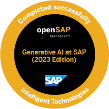
\includegraphics[width=1.5cm]{media/image23.png}}
  \end{minipage}

  \begin{itemize}
    \item Vendor: SAP, Score: 95.70\%, Attempt: First Attempt
    \item Verification Link: \href{https://open.sap.com/verify/xogaz-dimeh-rybiv-foser-teted}{\ul{Click here}}
  \end{itemize}

  \item
  \begin{minipage}[t]{\textwidth}
    \textbf{Certified Professional OCI Gen AI}
    \hfill
    \raisebox{-0.3\height}{\includegraphics[width=1.5cm]{media/50_Oracle_Cloud_Infrastructure.png}}
  \end{minipage}

  \begin{itemize}
    \item Vendor: Oracle University, Status: In-Progress
  \end{itemize}
  
  \item
    Certified AWS Code Whisper (AWS Q Developer)

    \begin{itemize}
      \item Vendor: Amazon Web Service (AWS), Status: Completed
      \item
        \begin{minipage}[t]{\textwidth}
          Category: Generative AI Developer
          \hfill
          \raisebox{-0.3\height}{
\includegraphics[width=1.2cm]{media/image25.png}}
        \end{minipage}
    \end{itemize}
  
  \item
    Microsoft Learn
  
    \begin{itemize}
    \item Badges: 114+
    \item Level: 11\textsuperscript{th} +
    \item Score: 179,125/227,799 XP+
    \item Trophies: 23+
    \item Transcript: \href{https://learn.microsoft.com/en-gb/users/mujahedh/transcript/d8k4jb84x69nm62}{\ul{Click here}}
    \end{itemize}
  
  \item
    Robotic Process Automation (RPA)
  \item
    Certified Adobe Master Collection
\end{itemize}

\begin{center}
  \textbf{PERSONAL DETAILS}
  \rule{\textwidth}{0.4pt}  % Full width of the page
\end{center}

\textbf{Name :} Mujahed Hussaini

\textbf{Passport :} S0001234

\textbf{Languages Known :} English, Hindi, Marathi, Arabic and Urdu.

\end{document}
